\label{•} 
\documentclass[11pt]{utalcaDoc}
\usepackage{graphicx}
\usepackage[utf8] {inputenc}
\usepackage[spanish]{babel}
\usepackage{verbatim}
\usepackage{algorithm}
\usepackage{algorithmic}

\title{{\bf Algoritmos y estructuras de datos}\\Tarea 1}
\author{Profesor: Rodrigo Paredes}
\date{Plazo: Viernes 20 de Abril de 2012. 0.5 puntos de descuento por d\'ia de atraso.}

\begin{document}
\renewcommand{\figurename}{Figura~}
\renewcommand{\tablename}{Tabla~}

%\maketitle
%
%\section{Objetivos}
% 
%En esta tarea se pretende que el alumno (1) se familiarice con los lenguajes
%de programaci'on C/C++ o Java, y (2) aprenda una metodolog'ia
%que le permita enfrentar un problema, construir un algoritmo que lo resuelva,
%definir un conjunto de casos de prueba apropiado para el problema en estudio
%y realizar los experimentos para validar el programa escrito.
%%que permitan analizar alguna caracter'istica
%%interesante del problema, realizar los experimentos y por 'ultimo modelar
%%el comportamiento de la caracter'istica de inter'es.
% 

%
%\section{Descripci'on de la tarea}
%
%Existen numerosas conjeturas sobre los n'umeros primos. En esta tarea trataremos
%de verificar experimentalmente si es que se cumplen o no tres de ellas, a saber:
%\begin{itemize}
%\item Conjetura Par de Goldbach: ``Todo n'umero natural par es la suma de a lo m'as
%dos primos''.
%\item Conjetura Impar de Goldbach: ``Todo n'umero natural impar mayor que 1
%es la suma de a lo m'as tres primos''.
%\item Conjetura de cinco primos: ``Todo n'umero natural es la suma de a lo m'as cinco primos distintos''.
%\end{itemize}
%
%
%El objetivo de la tarea es verificar experimentalmente las conjeturas. Para eso
%ustedes implementar'an un programa en C/C++/Java que obedezca la
%siguiente l'inea de comandos:\\
%\verb$tarea1 --conjetura [1|2|3] -n N -v$
%
%donde el primer par de argumentos (\verb$--conjetura [1|2|3]$) indica que conjetura
%est'an verificando, el segundo par (\verb|-n N|) para que valor de $N$ lo est'an haciendo
%y \verb|-v| es una ejecuci'on con muchos comentarios con fines de depuraci'on.
%Noten que se prueba cada conjetura por separado. Por ejemplo, para probar la
%conjetura impar de Goldbach, para el primer mill'on de n'umeros y sin activar
%la opci'on verbosa, la invocaci'on en la l'inea de comandos ser'ia:\\
%\verb$tarea1 --conjetura 2 -n 1000000$
%
%Para esto ustedes deber'an manejar una estructura que permita administrar a los n'umeros
%primos, y luego implementar algoritmos iterativos o recursivos para verificar la
%conjetura para cada valor de $n$ entre 2 y $N$.
%
%Si la conjetura se cumple, el programa imprime:\\
%\noindent \verb|La conjetura XXX se cumple|
%
%En caso contrario, imprime:
%\begin{verbatim}
%La conjetura XXX no se cumple
%Numeros que la fallan: N1, N2, ...
%\end{verbatim}
%
%En que \verb|XXX| es el n'umero o texto de la conjetura y \verb|N1, N2, ...| son los
%n'umeros que hacen fallar la conjetura, de haberlos.
%
%
%\textbf{Pruebas preliminares.} Para poder verificar que sus algoritmos est'en
%operando correctamente, ustedes implementar'an una variante verbosa
%que les permitir'a chequear manualmente (esta opci'on tambi'en ser'a usada
%en el proceso de correcci'on de la presente tarea). En la variante verbosa su
%programa tendr'a que mostrar la tabla de n'umeros primos desde 2 hasta $N$.
%
%En la opci'on verbosa tienen que mostrar la tabla de primos. El formato de
%salida es de acuerdo al siguiente ejemplo:
%\begin{verbatim}
%tarea1 --conjetura 2 -n 20 -v
%TABLA DE PRIMOS
%2
%3
%5
%7
%11
%13
%17
%19
%La conjetura impar de Goldbach se cumple
%\end{verbatim}
%
%
%
%\textbf{Experimentaci'on.} Tendr'an que ejecutar el programa con valores grandes
%de $N$. Por razones de uso de memoria, vuestro programa tendr'ia que poder ejecutarse
%con valores de $N$ que lleguen a $10^{9}$ para cada una de las tres conjeturas.
%
%En el informe indiquen como var'ian los tiempos de computo a medida que aumenta
%$N$ en una decada de estudio (por ejemplo, de $10^{8}$ hasta $10^{9}$).
%
%La tarea tendr'a las siguientes penalizaciones que se aplican a la nota total de la tarea.
%
%\begin{center}
%\begin{tabular}{|c|c|c|c|c|c|}
%\hline
%rango de $N$ & $[10^{9}, \infty)$ & $[10^{8}, 10^{9})$ & $[10^{7}, 10^{8})$ & $[10^{6}, 10^{7})$ & $[1, 10^{6})$\\ \hline 
%penalizaci'on & sin penalizaci'on & -0.5 pts & -1 pt & -2 pts & -4 pts \\ \hline
%\end{tabular}
%\end{center}

%\section{Pruebas}
%
%
%\section{Restricciones}
%
%\begin{itemize}
%\item Los programas debe ser escritos en C, C++ o Java.
%\item Plazo de entrega: Viernes 20 de Abril de 2012. 0.5 puntos de descuento por d'ia de atraso.
%\item Queda prohibido utilizar bibliotecas o clases preconstruidas en el lenguaje
%    que implementen operaciones no est'andar sobre arreglos. Tampoco se puede
%    utilizar clases que administren arreglos (por ejemplo, se prohibe el uso de HashMaps
%    u otras). USTED DEBE IMPLEMENTAR TODO.
%\item La tarea es individual.
%\item Para la tarea tienen que entregar un informe de resultados junto al c'odigo
%    fuente (el programa que implementa la tarea). No se aceptan c'odigos sin
%    informe ni informes sin c'odigo.
%\item Si la tarea no compila tiene nota 1.0 tanto en el c'odigo como en el informe.
%\item Cualquier falta a las restricciones anteriores invalida irrevocablemente
%la tarea.
%\end{itemize}
%
%
%\section{Indicaciones}
%
%%Se recomienda Java.
%
%Si el informe de la tarea se escribe en \LaTeX, tiene un punto extra
%en el informe.
%
%
%\section{Ponderaci'on}
%
%El informe equivale a un 35\% de la nota de tarea.
%    
%El c'odigo equivale a un 65\% de la nota de tarea.
%
%
%\section{Entrega de la tarea}
%
%La entrega de la tarea debe incluir (1) el c'odigo del programa que resuelve
%la tarea y (2) un informe escrito donde se describa y documente el programa
%entregado, y se incluyan ejemplos de entradas y salidas. La entrega de la tarea
%se realizar'a a trav'es de la plataforma {\tt lms.educandus.cl} hasta las 23:55 del d'ia
%del plazo final. Generen un 'unico archivo que contenga tanto el informe como
%los c'odigos para compilar. Tambi'en se solicita que se adjunte un archivo
%README que explique c'omo compilar la tarea.
%     
%El contenido del informe debe seguir la siguiente pauta com'un para todas las tareas: 

%Portada. El formato de la portada se muestra a continuaci'on:

\begin{figure}[H]
\epsffile{utalca.eps} %{\epsfxsize16mm \epsffile{utalca.eps}} %
\rlap{\kern 4mm \lower -9.5mm \hbox to0pt{{\Large \sc Universidad~~de~~Talca}\hfill}}%
\rlap{\kern 4mm \lower -5mm \hbox to0pt{\Large \sc Facultad~~de~~Ingenier\'ia\hfill}}%
\rlap{\kern 4mm \lower -1mm \hbox to0pt{%
  {\large \sc Departamento~~de~~Ciencias~~de~~la~~Computaci\'on}\hfill}}%

\vspace{8cm}

\centerline{\huge \bf Informe Tarea 2}
\vspace{0.8cm}
\centerline{\Large \bf Simulacion de colas en un banco}

\vspace{8cm}

\hfill \begin{tabular}{ll}
Fecha:  & Martes, 5 de Junio del 2012\\
Autor:  & Erik Andres Regla Torres\\
e-mail: & eregla09@alumnos.utalca.cl

\end{tabular}

\label{fig1}
\end{figure}

\section{Introducci'on}

\section{An'alisis del problema} El problema consiste basicamente en solucionar el ordenamiento de un conjunto de datos directamente en la memoria auxiliar (disco duro) intentando utlizar una cantidad minima de memoria física.\\

Como estructuras necesarias, se plantea el uso de una cola de prioridad, una cola simple, y una estructura basica para almacenar la informacion de cada una de las personas. Abondar en como esta compuesta cada una de ellas, es trivial ya que es algo visto en la clase.\\

\section{Soluci'on del problema}
  \subsection{Algoritmo de soluci'on} Primero, dentro de el programa solicitado, comienza con la etapa de verificacion. Se validan los argumentos entregados de modo que estos no produzcan algun error propagable dentro de la ejecucion. De no ser valido algun argumento, el programa termina su ejecucion informandole al usuario del error.\\
  Luego comienza la etapa de la ejecucion propiamente tal. La clase ``Simulador.java'' se encarga de iniciar la ejecucion de la simulacion en el mismo constructor de la clase. Este configura las variables de la ejecucion, y luego define el tipo de cola a utilizar. Luego entra a un ciclo infinito, que dependiendo del retardo que tenga provoca que la simulacion tome mas o menos tiempo.\\
  
  Cada vez que se entra al ciclo, imprime las estadisticas correspondientes a la simulacion, acto seguido, verifica si la simulacion esta corriendo dentro del tiempo especificado del usuario. De ser asi, entonces al final de los calculos, realiza la extraccion de una persona de la cola. Idependiente de que lo mencionado anteriormente ocurra, se extrae una persona de la cola,  y se le consume el tiempo.\\
  
  Una vez que el tiempo nesesario para llevar a cabos sus operaciones se ha acabado, esta persona sale de la cola, y entra otra. De no haber ninguna, se pasa a la siguiente iteracion. Cada iteracion equivale a un segundo de simulacion.
  
  \subsection{Diagrama de Estados}
  		\begin{figure}[H]
  			\centering
    		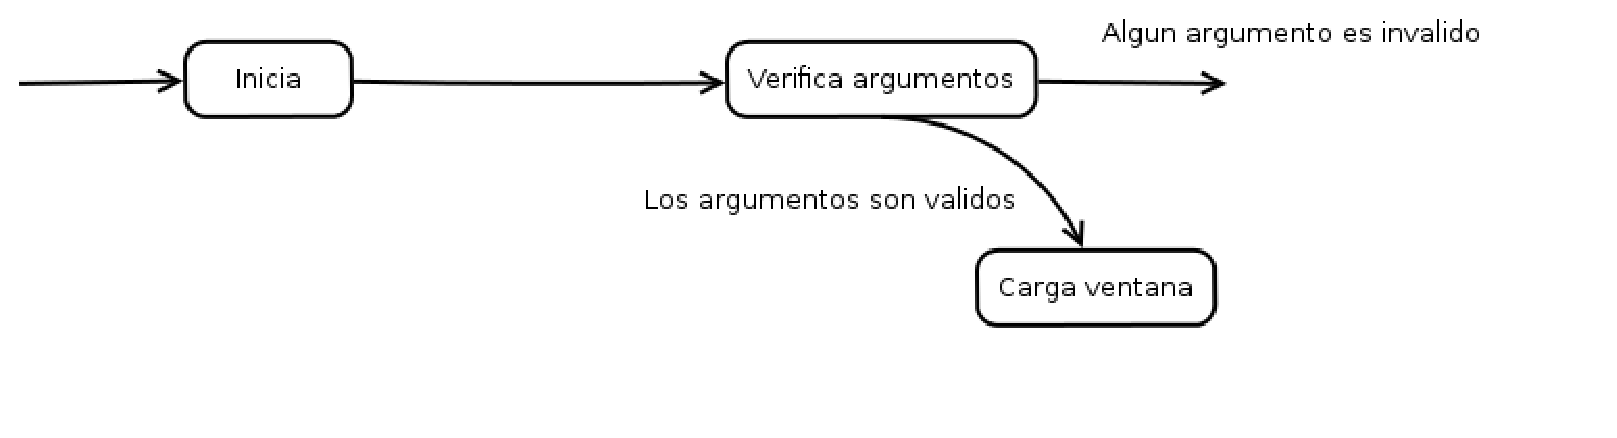
\includegraphics[width=0.85\textwidth]{etapa1}
  			\caption{Inicio}
		\end{figure}
  		\begin{figure}[H]
  			\centering
    		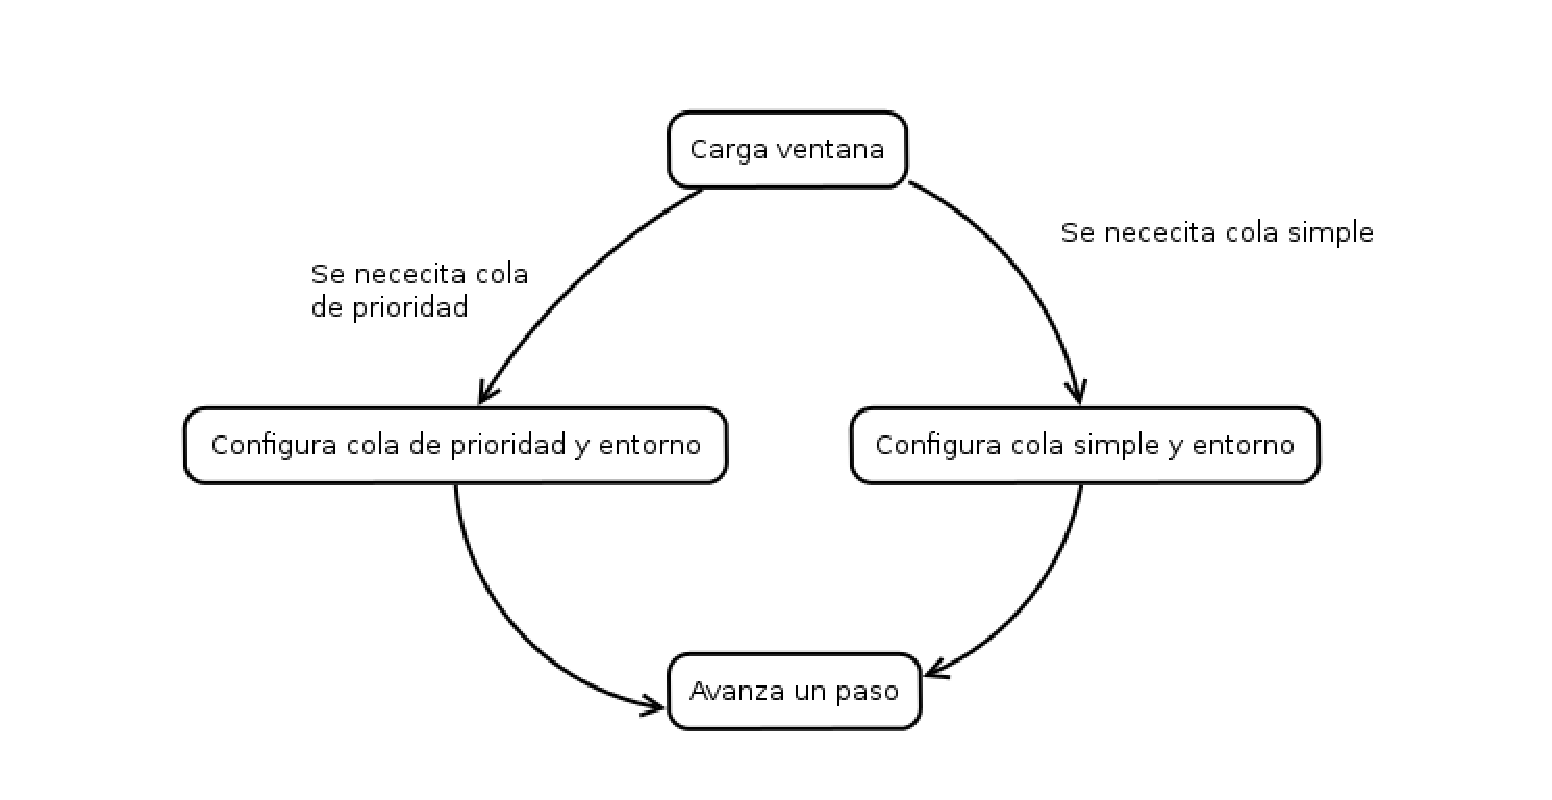
\includegraphics[width=0.85\textwidth]{etapa2}
  			\caption{Configuracion}
		\end{figure}
  		\begin{figure}[H]
  			\centering
    		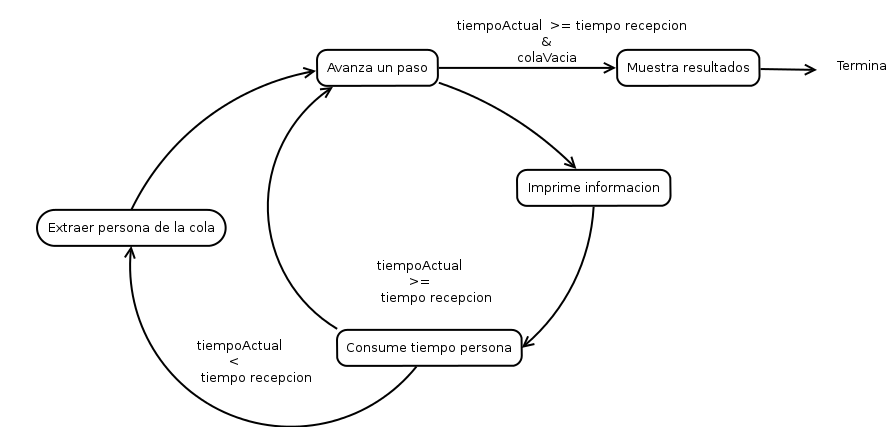
\includegraphics[width=0.85\textwidth]{etapa3}
  			\caption{Simulacion}
		\end{figure}
  
  \subsection{Dise\~no} Explicitar las Pre y Post condiciones consideradas,
  mostrar los invariantes empleados.

  \subsection{Implementaci'on}
	\begin{algorithm}[H]                      % enter the algorithm environment
	\caption{computo de pasos para la simulacion}          % give the algorithm a caption
	\label{alg1}                           % and a label for \ref{} commands later in the document
	\begin{algorithmic}                    % enter the algorithmic environment
	    \REQUIRE cola no vacia
	    \ENSURE que todas las personas de la cola hayan sido atendidas
	    
	    \STATE $imprimirInformacion()$
	    \STATE $step \Leftarrow step + 1$
	    
		\IF{$step > maxTime$}
	    	\IF{$actual = null$}
	    		\RETURN \FALSE
	    	\ENDIF
	    	\COMMENT en caso de que la persona haya terminado lo que tenia que hacer
	    	\IF{$actual.stepTimeOut()$}
	    		\STATE $actual \leftarrow siguiente$
	    		\STATE $siguiente \leftarrow popCurrent()$
	    	\ENDIF
	    	\IF{$siguiente = null$}
	    		\RETURN \FALSE
	    	\ENDIF
	    \ELSE
	    	\IF{$siguiente = null$}
	    		\STATE $siguiente \leftarrow popCurrent()$
	    	\ENDIF
	    	\IF{$actual != null$}
  		    	\IF{$actual.stepTimeOut()$}
		    		\STATE $actual \leftarrow siguiente$
		    		\STATE $siguiente \leftarrow popCurrent()$
	    		\ENDIF
	    	\ENDIF
	    	\IF{$siguiente = null$}
	    		\RETURN \FALSE
	    	\ENDIF
	    	
	    	\IF{$step\%60 = 0$}
	    		\STATE $pushNew()$
	    	\ENDIF
	    \ENDIF
    	\IF{$step\%60 = 0$}
    		\STATE $imprimeInformacion()$
  	 	\ENDIF
		\RETURN \TRUE	
	\end{algorithmic}
	\end{algorithm}
  
  \subsection{Modo de uso} Se entrega un proyecto de netbeans, compilante con la version 7.0.1 RC2. Para poder compilar usando este IDE, se recomienda importar el proyecto. Caso contrario, se sugiere ejecutar la compilacion desde el directorio raiz de las fuentes.

\section{Pruebas} Se debe mostrar las pruebas realizadas y sus resultados.
%Se debe se\~nalar claramente cual es la llamada al programa y su salida.
El n'umero de pruebas puede variar dependiendo del problema
En esta secci'on debe incluir las tablas y gr'aficos necesarios solicitados,
y el an'alisis de los resultados. En este cap'itulo adjunten las conclusiones
obtenidas de los resultados de la tarea.
%En general tres pruebas es suficiente.

\section{Anexos} De ser necesario, cualquier informaci'on adicional se debe
agregar en los anexos y debe ser referenciada en alguna secci'on del
informe de la tarea. Dentro de los anexos se puede incluir un listado con
el programa completo que efectivamente fue compilado.

\end{document}
